\section{From Principles to Constraints}
\label{sec:encoding}

A verbal principle from Section~\ref{sec:principles} enters at the top of this section
and a routing leaves at the bottom. Every step is stated in the form the solver receives,
and each design choice is given with the alternative it was chosen over.

\subsection{The routing model}
\label{sec:routing-model}

Airspace is discretised into $M$ ground tiles $\stations = \{1,\dots,M\}$, each standing
for one community with its own ambient noise level and demographic attributes. Movement
is given by an adjacency matrix $A \in \{0,1\}^{M \times M}$, \emph{with self-loops}
($A_{mm}=1$) so an aircraft may hold position; Section~\ref{sec:softT} explains why those
are mandatory rather than convenient. A fleet of $N$ aircraft
$\aircraft = \{1,\dots,N\}$ is routed over $T$ discrete timesteps
$\steps = \{0,\dots,T-1\}$, aircraft $i$ having origin $s_i$, destination $e_i$, and a
multiplier $\mu_i \in \mathbb{Z}_{>0}$ giving how many physical aircraft the variable
represents ($\mu_i = 1$ routes every flight independently; larger values pack a corridor
into one variable at the cost of forcing those flights onto a common path).

The decision variables are integer locations
\begin{equation}
L_{i,t} \in \stations, \qquad i \in \aircraft,\ t \in \steps,
\end{equation}
subject to origin pinning and adjacency-respecting motion:
\begin{align}
L_{i,0} &= s_i, \label{eq:start}\\
L_{i,t} = m &\Rightarrow \bigvee_{m' :\, A_{mm'} = 1} L_{i,t+1} = m'. \label{eq:move}
\end{align}
A timestep is a fixed wall-clock interval (\SI{180}{\second} in our instantiation), which
is what converts a dimensionless hop count into an exposure duration.

\subsection{When an aircraft is audible}
\label{sec:active}

A parked aircraft makes no noise, and neither does one that has landed. Encoding this is
not cosmetic: it determines which tiles a flight is charged for. Three Boolean families
track it, for each $i \in \aircraft$:
\begin{align}
\mathrm{mv}_{i,0} &= \bot, &
\mathrm{mv}_{i,t} &= \mathrm{mv}_{i,t-1} \vee (L_{i,t} \neq s_i), \label{eq:mv}\\
\mathrm{ha}_{i,0} &= [s_i = e_i], &
\mathrm{ha}_{i,t} &= \mathrm{ha}_{i,t-1} \vee (L_{i,t} = e_i), \label{eq:ha}\\
\mathrm{ac}_{i,0} &= \bot, &
\mathrm{ac}_{i,t} &= \mathrm{mv}_{i,t} \wedge \neg\,\mathrm{ha}_{i,t-1}. \label{eq:ac}
\end{align}
Both $\mathrm{mv}$ (``has departed'') and $\mathrm{ha}$ (``has arrived'') are sticky.
The activity flag $\mathrm{ac}_{i,t}$ gates on $\mathrm{ha}_{i,t-1}$, not
$\mathrm{ha}_{i,t}$, so an aircraft \emph{is} counted on the timestep it touches down ---
the landing is audible --- and silent from the next step onward.

Two consequences are easy to get wrong. An origin tile never accumulates noise from
flights that have not departed, so a corridor whose whole fleet shares one vertiport does
not thereby violate a cap. And waiting at the origin is free under every noise objective,
so only an arrival-time term gives aircraft any reason to depart promptly.

The weighted occupancy of tile $m$ at time $t$ is then
\begin{equation}
c_{m,t} \;=\; \sum_{i \in \aircraft} \mu_i \cdot
  \bigl[\,L_{i,t} = m \ \wedge\ \mathrm{ac}_{i,t}\,\bigr].
\label{eq:count}
\end{equation}

\subsection{The noise model}
\label{sec:noise}

Aircraft noise adds to ambient noise in \emph{energy}, not in decibels. With ambient
level $b_m$ at tile $m$ and a per-aircraft source level $\alpha$, the increase caused by
$n$ simultaneous overflights is
\begin{equation}
\dbinc_m(n) \;=\; 10\log_{10}\!\Bigl(10^{b_m/10} + n\,10^{\alpha/10}\Bigr) - b_m
          \;=\; 10\log_{10}\!\Bigl(1 + n\,10^{(\alpha - b_m)/10}\Bigr).
\label{eq:db}
\end{equation}
Every fairness statement in this paper is made about $\dbinc$, the \emph{added} noise,
rather than about the absolute level $b_m + \dbinc_m(n)$. That choice is itself
normative and we return to it in Section~\ref{sec:results}.

Equation~\eqref{eq:db} has three properties that drive nearly every result reported
later, and they are properties of acoustics rather than of our encoding:
\begin{enumerate}
\item $\dbinc_m$ is \textbf{strictly increasing} in $n$. Bounding the count therefore
      bounds the noise exactly, which we exploit in \eqref{eq:dcap}.
\item $\dbinc_m$ is \textbf{strictly concave} in $n$. The first aircraft over a quiet
      tile costs far more than the tenth, so \emph{concentrating} traffic is cheaper
      than spreading it whenever the objective is expressed in decibels.
\item $\dbinc_m$ is \textbf{decreasing in the ambient level} $b_m$. At
      $\alpha = \SI{45}{\dBA}$, one aircraft adds \SI{3.01}{\dB} over a \SI{45}{\dBA}
      tile but only \SI{0.04}{\dB} over a \SI{65}{\dBA} one --- a ratio of about $70$.
      Already-loud communities are, in this metric, almost free to overfly.
\end{enumerate}

Because Z3's integer arithmetic cannot represent \eqref{eq:db}, we tabulate it at
centi-decibel resolution, $\tilde\dbinc_m(n) = \mathrm{round}(100\,\dbinc_m(n))$, and
encode the table as a nested conditional over the reachable counts. Rounding is not
free: it destroys concavity locally (the row for $b_m = \SI{65}{\dBA}$ reads
$0,4,9,13,17,21$, whose first differences $4,5,4,4,4$ are not monotone even though the
true differences $4.32,4.28,4.24$ are), which matters when a bound over the table must
be computed exactly --- see Section~\ref{sec:normalisation}.

\subsection{The two hard noise constraints}
\label{sec:hard}

Two caps are available, and Section~\ref{sec:mapping} assigns them to principles.

\paragraph{Absolute cap $D$} No tile's added noise may exceed $D$ at any time. Rather
than assert $\tilde\dbinc_m(c_{m,t}) \le \tilde D$ directly, we precompute the
per-tile capacity
\begin{equation}
\capm_m \;=\; \max\{\, n : \tilde\dbinc_m(n) \le \tilde D \,\}
\label{eq:cap}
\end{equation}
and assert the equivalent bound on the count,
\begin{equation}
0 \;\le\; c_{m,t} \;\le\; \capm_m .
\label{eq:dcap}
\end{equation}
Equivalence is exactly property~1 above. This costs $M$ constraints per timestep instead
of a conditional table, and it also shortens every conditional elsewhere in the model,
since counts above $\capm_m$ are now unreachable and their branches can be omitted.

Fig.~\ref{fig:capacity} makes the practical content of \eqref{eq:cap} visible, and it is
the single most consequential plot in the paper: a cap on \emph{added} noise makes quiet
tiles nearly unusable while leaving loud ones effectively unconstrained.

\begin{figure}[t]
\centering
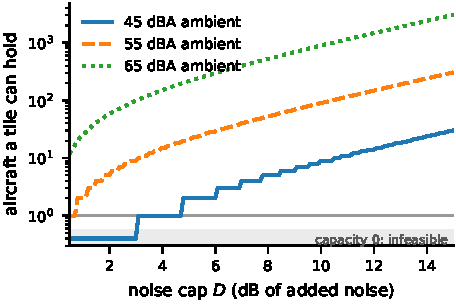
\includegraphics{figs/capacity.pdf}
\caption{Simultaneous overflights a community can absorb under a cap $D$ on
\emph{added} noise, by ambient level, from \eqref{eq:capclosed}. The cap is
baseline-independent; the capacity it implies is not. At $D=\SI{3}{\dB}$ a
\SI{45}{\dBA} community can host no aircraft at all, while a \SI{65}{\dBA} one can
host 99.}
\label{fig:capacity}
\end{figure}

\paragraph{Disparity cap $U$} At any timestep, the spread of added noise across tiles
may not exceed $U$. The direct statement is pairwise,
\begin{equation}
\bigl|\dbinc_{m_1}(c_{m_1,t}) - \dbinc_{m_2}(c_{m_2,t})\bigr| \le U
\quad \forall\, m_1,m_2,t ,
\label{eq:upair}
\end{equation}
which requires a conditional table over every \emph{ordered pair} of tiles and every
count value --- $O(M^2 \capm)$ implications per timestep. We instead use the identity
\begin{equation}
\eqref{eq:upair} \iff \max_m \dbinc_m(c_{m,t}) - \min_m \dbinc_m(c_{m,t}) \le U
\end{equation}
and introduce two auxiliary integers per timestep:
\begin{equation}
\overline{d}_t \ge \tilde\dbinc_m(c_{m,t}),\quad
\underline{d}_t \le \tilde\dbinc_m(c_{m,t}) \ \ \forall m, \quad
\overline{d}_t - \underline{d}_t \le \tilde U .
\label{eq:ucap}
\end{equation}
This is sound and complete. Soundness: $\overline{d}_t$ is forced at or above the true
maximum and $\underline{d}_t$ at or below the true minimum, so bounding their difference
bounds the true spread. Completeness: any assignment whose true spread fits within $U$
is satisfiable by setting the auxiliaries to the actual extremes. The cost falls to
$2M+1$ constraints per timestep, and the conditionals it refers to are the ones the
objective terms need anyway, so the disparity cap adds no new nonlinear terms at all.

\begin{table}[t]
\centering
\caption{The two disparity encodings, built on an otherwise identical phase-2 model and timed. Both state the same constraint and agree on the objective at every size. The pairwise form needs two orders of magnitude more assertions and takes correspondingly longer to \emph{build}, but it \emph{solves} $6$--$9\times$ faster --- so the max/min encoding's advantage is in construction, and it decays from $3.2\times$ on total time at $N{=}6$ to parity at $N{=}16$. Single runs on an idle machine; the solve times at $N{=}6$ are under a second and should be read as indicative.}
\label{tab:pairwise}
\begin{tabular}{r rr rr rr}
\toprule
\multirow{2}{*}{$N$} & \multicolumn{2}{c}{max/min} & \multicolumn{2}{c}{pairwise} & \multicolumn{2}{c}{ratio} \\
\cmidrule(lr){2-3}\cmidrule(lr){4-5}\cmidrule(lr){6-7}
 & constr. & solve (s) & constr. & solve (s) & solve & total \\
\midrule
6 & 306 & 0.64 & 25,200 & 0.12 & $0.19\times$ & $3.22\times$ \\
8 & 306 & 1.28 & 32,400 & 0.20 & $0.16\times$ & $2.31\times$ \\
14 & 306 & 4.47 & 48,240 & 0.47 & $0.11\times$ & $1.17\times$ \\
16 & 306 & 6.11 & 53,136 & 0.72 & $0.12\times$ & $1.00\times$ \\
\bottomrule
\end{tabular}
\end{table}


The constraint counts differ by two orders of magnitude, and we initially reported that
ratio as though it were a speedup. Building both encodings on an otherwise identical
model and timing them says otherwise (Table~\ref{tab:pairwise}). The two agree on the
objective at every size, confirming they state the same constraint. But the pairwise
encoding \emph{solves} $6$--$9\times$ \textbf{faster}: giving Z3 the disparity relation
explicitly, rather than through two auxiliary variables it must reason about, evidently
helps its search. What max/min buys is \emph{construction} time --- 306 assertions
against tens of thousands --- and that advantage decays with fleet size, from
$3.2\times$ on total time at $N=6$ to exactly $1.0\times$ at $N=16$. Extrapolating the
trend, the pairwise form would win outright at the fleet sizes we most care about.

We report this because the honest conclusion contradicts the one we started with. The
max/min encoding is worth keeping at workshop scale, where a solve is dominated by
construction and the tool must feel responsive; it is not what makes these problems
tractable, and the constraint-count ratio was never evidence that it was. Constraint
counts are a proxy for encoding cost, not for search cost, and the two came apart here in
the direction opposite to the intuition.

\subsection{Horizon selection and the two-phase solve}
\label{sec:softT}

$T$ is not given. Too small and the instance is spuriously infeasible; too large and
every extra timestep replicates the entire noise encoding for all $M$ tiles. We
therefore solve in two phases.

\emph{Phase 1} finds the smallest feasible horizon. A lower bound $T_{\min}$ comes from
a breadth-first search per aircraft restricted to \emph{$D$-admissible} tiles, those
with $\capm_m \ge \mu_i$; this is a sound necessary condition because it ignores all
interaction between aircraft and so can only under-constrain. The encoding is then built
once at $T_{\min}$ and extended by a single timestep per iteration, with the destination
pins $L_{i,T-1} = e_i$ asserted as \emph{assumption literals}. This lets the unsat core
distinguish the two ways an instance can fail: if no destination assumption appears in
the core, the conflict is structural and no horizon will ever help, so the search stops
immediately instead of grinding to its cap.

\emph{Phase 2} fixes the horizon and optimises. Under a \emph{soft} horizon the phase-2
horizon is set above $T_{\min}$, giving aircraft room to stagger their arrivals rather
than all being airborne simultaneously; arrival is then made sticky,
\begin{equation}
\mathrm{ha}_{i,t} \Rightarrow L_{i,t+1} = e_i ,
\label{eq:sticky}
\end{equation}
so an aircraft that lands early stays landed instead of drifting. Constraint
\eqref{eq:sticky} is why self-loops in $A$ are mandatory: without $A_{e_ie_i}=1$ a
landed aircraft would have no legal move and the instance would be trivially
unsatisfiable.

\subsection{Mapping the five principles}
\label{sec:mapping}

Table~\ref{tab:mapping} summarises the translation; the five subsections that follow give
each principle separately, since what each one needs from the model differs more than a
shared notation suggests. Throughout, $P \subseteq \stations$ is a protected set, $w_m$ a
per-tile transit weight, and $\pi_m$ a per-tile price. Every objective is minimised.

%% Hand-written (unlike the rest of tables/, which analyze.py generates).
%% This is the paper's central claim about the encoding, not a measurement.
\begin{table*}[t]
\centering
\caption{The five principles as constraints. ``Form'' is whether the principle's own
statement is a satisfaction condition or an optimisation; ``Encoded as'' is what our
solver receives. The one row where these disagree is Equal, and
Section~\ref{sec:mismatch} measures what that disagreement costs. $\ell$ is the
user-selected decibel limit, $P$ the protected set, $\pi_m$ the benefit-derived price
of \eqref{eq:price}, and $\infty$ a cap set wide enough to be unreachable.}
\label{tab:mapping}
\begin{tabular}{llllc}
\toprule
Principle & Statement in this domain & Form & Encoded as & Objective? \\
\midrule
Equal &
  added noise as equal as possible across communities &
  optimisation &
  hard cap $U \le \ell$ (and $D \le \ell$) &
  no \\
Sufficientarian &
  no community's noise exceeds a stated threshold &
  satisfaction &
  hard cap $D \le \ell$, $U \le \infty$ &
  no \\
Prioritarian &
  the already most-burdened receive the least additional noise &
  optimisation &
  $\min J_{\mathrm{prior}} = \sum_{t}\sum_{p \in P} \tilde\dbinc_p(c_{p,t})$ &
  yes \\
Utilitarian &
  the summed added noise over all communities is lowest &
  optimisation &
  $\min J_{\mathrm{util}} = \sum_{t}\sum_{m} w_m \tilde\dbinc_m(c_{m,t})$ &
  yes \\
Proportional &
  those who benefit most from the network carry more of its noise &
  optimisation &
  $\min J_{\mathrm{prop}} = \sum_{t}\sum_{m} \pi_m\,\tilde\dbinc_m(c_{m,t})$ &
  yes \\
\bottomrule
\end{tabular}
\end{table*}


\subsubsection{Equal}
\label{sec:enc-equal}
Equal constrains differences between communities, so it is the one principle that needs a
quantity no single community possesses. We bound the spread of added noise at every
timestep,
\begin{equation}
\max_m \dbinc_m(c_{m,t}) - \min_m \dbinc_m(c_{m,t}) \;\le\; \ell
\quad \forall t ,
\label{eq:enc-equal}
\end{equation}
which is the disparity cap $U = \ell$ of \eqref{eq:ucap}, and we contribute no objective
term. This takes the satisfaction reading of Equal identified in
Section~\ref{sec:p-equal}. It is the cheaper reading --- \eqref{eq:ucap} costs $2M+1$
linear constraints per timestep, against an optimisation over $\max_m - \min_m$ which
would add a further objective tier --- and it is the reading the deployed tool takes.
Section~\ref{sec:mismatch} measures what it costs, and the cost is not small.

\subsubsection{Sufficientarian}
\label{sec:enc-suff}
Sufficientarian constrains each community's own increase against a threshold, with no
reference to any other community:
\begin{equation}
\dbinc_m(c_{m,t}) \;\le\; \ell \quad \forall m,t ,
\label{eq:enc-suff}
\end{equation}
which is the absolute cap $D = \ell$, enforced through the count bound \eqref{eq:dcap}.
Again no objective term, and here that is faithful rather than a compromise:
Sufficientarianism is natively a satisfaction condition and is genuinely silent among
distributions that clear the threshold. Of the five this is the only principle whose form
survives the encoding untouched.

\subsubsection{Prioritarian}
\label{sec:enc-prior}
Prioritarian needs an input the noise model does not contain --- an identification of the
already worst-off --- which enters as an explicit protected set $P$. It then minimises
the noise those communities receive:
\begin{equation}
J_{\mathrm{prior}} \;=\; \sum_{t}\sum_{p \in P} \tilde\dbinc_p(c_{p,t}) .
\label{eq:jprior}
\end{equation}
Two properties follow from the shape of \eqref{eq:jprior} and both are visible in
Section~\ref{sec:degeneracy}. It is bounded below by zero and \emph{attains} zero whenever
a routing exists that never overflies $P$, after which it expresses no further
preference --- so it behaves as a hard exclusion wearing an objective's clothing. And
because it is silent about every community outside $P$, it says nothing about where the
displaced traffic goes.

We choose $P$ as the three loudest non-vertiport communities, following the source
document's ``regions that presently and historically bear the greatest noise burden from
existing transportation infrastructure''. Vertiports are excluded because every flight
must land at one, which would make the objective unsatisfiable rather than binding.

\subsubsection{Utilitarian}
\label{sec:enc-util}
Utilitarian aggregates, so it sums the added noise over every community and timestep:
\begin{equation}
J_{\mathrm{util}} \;=\; \sum_{t}\sum_{m} w_m\,\tilde\dbinc_m(c_{m,t}) ,
\label{eq:jutil}
\end{equation}
with $w_m \equiv 1$ unless the deployment weights communities by population. This is the
most direct of the five translations --- the principle names a sum, and the encoding is
that sum --- and it inherits the principle's indifference to distribution exactly:
\eqref{eq:jutil} cannot distinguish one community bearing $20$ units from twenty bearing
one. Combined with the concavity and baseline-dependence of \eqref{eq:db}, that
indifference has consequences we quantify in Section~\ref{sec:concavity}.

\subsubsection{Proportional}
\label{sec:enc-prop}
Proportional is relational: it ties burden to benefit, and benefit is not in the noise
model at all. Section~\ref{sec:proportional-encoding} constructs a per-tile price $\pi_m$
from participants' own ranking of what confers benefit; given it, the objective is
\begin{equation}
J_{\mathrm{prop}} \;=\; \sum_{t}\sum_{m} \pi_m\,\beta_{m,t} ,
\label{eq:jprop}
\end{equation}
where $\beta_{m,t}$ is a burden measure defined below. Because $\pi_m$ is
\emph{constructed} rather than measured, this is the one principle whose encoding embeds
a second set of contestable judgements on top of the principle itself --- which is why we
make the construction an explicit input rather than a constant.

\subsubsection{Arrival time, which is not a principle}
\label{sec:enc-time}
Independently of the five, aircraft should not loiter. We count pre-arrival
aircraft-timesteps,
\begin{equation}
J_{\mathrm{time}} \;=\; \sum_{i}\sum_{t} [\,\neg\,\mathrm{ha}_{i,t}\,] ,
\label{eq:jtime}
\end{equation}
a proxy for total travel time. This is an efficiency term, not a fairness one, and
Section~\ref{sec:normalisation} explains why it is kept strictly subordinate to whichever
principle is selected.

\subsection{Constructing ``benefit'' for the Proportional principle}
\label{sec:proportional-encoding}

Proportional requires a quantity the noise model does not contain. We construct it
explicitly, as a price $\pi_m$ that the objective pays for each unit of burden borne by
tile $m$; minimising $J_{\mathrm{prop}}$ therefore pushes traffic \emph{toward} cheap
tiles, so a low price means ``benefits from the system, should carry noise'' and a high
price means ``protected''.

Participants rank $F$ plain-language factors --- in our instantiation income, current
ambient level, distance to the nearest vertiport, and population. Each factor $f$ scores
every tile on a common scale $\sigma_f(m) \in [0,\Sigma]$ where $0$ means ``overfly
freely'' and $\Sigma$ means ``protect''. A rank order induces weights $\rho_f$ summing
to one, and
\begin{equation}
\pi_m \;=\; \gamma^{\;\sum_{f} \rho_f\,\sigma_f(m)}
       \;=\; \prod_{f} \gamma^{\,\rho_f \sigma_f(m)} ,
\label{eq:price}
\end{equation}
with base $\gamma$. The product form is deliberate: each factor contributes its own
multiplicative factor, so a price reads back as the separate contribution of each ranked
choice rather than one opaque number. Since $\sum_f \rho_f = 1$ and
$\sigma_f \in [0,\Sigma]$, the price stays in $[1,\gamma^\Sigma]$ however participants
rank. The distance factor's \emph{sign} is the principle: proximity to a vertiport scores
as cheap, because the tiles nearest a vertiport enjoy the access and so under
benefit-carries-burden are the ones that should pay. A prototype that scored proximity as
deserving protection was implementing the opposite principle.

The burden measure $\beta_{m,t}$ admits two non-interchangeable choices. \emph{Occupancy},
$\beta_{m,t} = c_{m,t}$, charges each aircraft-timestep that tile's price linearly; being
separable across aircraft it is far cheaper to optimise. \emph{Decibel},
$\beta_{m,t} = \tilde\dbinc_m(c_{m,t})$, charges the noise the community actually
experiences --- the more defensible reading, and our default. The decibel form inherits
both awkward properties of \eqref{eq:db}: concavity makes the objective \emph{prefer} to
concentrate traffic, and baseline-dependence applies the $\approx\!70\times$ gradient
toward loud tiles on top of whatever ambient preference participants expressed,
double-counting a factor they were asked to rank. We flag the trade rather than resolving
it: which reading is correct is a normative question our measurements can inform but not
settle.

\subsection{Normalisation and the priority between constraints}
\label{sec:normalisation}

The terms in \eqref{eq:jutil}--\eqref{eq:jtime} have incommensurable units --- summed
centi-decibels, priced occupancy, aircraft-timesteps. Each is therefore divided by an
upper bound on its own value, so that a stated weight of $1.0$ means the same thing
across terms:
\begin{equation}
\hat{J}_k = J_k / J_k^{\max}, \qquad
J_{\mathrm{tier1}} = \sum_k \omega_k \hat{J}_k .
\end{equation}
These bounds must be \emph{tight}, not merely valid: a loose divisor produces no error,
it silently shrinks a term's reachable range, so a weight the user set to $1.0$ behaves
like a much smaller number and the routing stops responding to it. The obvious bound for
$J_{\mathrm{prop}}$ --- every tile simultaneously carrying the whole fleet --- needs
$M\sum_i \mu_i$ aircraft when only $\sum_i \mu_i$ exist, and overstates the attainable
maximum by $16.4\times$ here. We instead compute the exact single-timestep maximum by
bounded-knapsack dynamic programming, rather than greedy marginal allocation, precisely
because rounding destroyed concavity (Section~\ref{sec:noise}) and greedy would
under-estimate --- the harmful direction.

\paragraph{Priority.} Folding $J_{\mathrm{time}}$ into the same weighted sum as the
principle terms makes the outcome depend on how tight each normalising bound happens to
be, which is a property of the bounds rather than of the ethics. An earlier version of
this system did exactly that: instrumenting it showed the time term occupying $68.8\%$ of
its normalised range against the utilitarian term's $2.2\%$, so with every stated weight
at $1.0$ the solver was in effect minimising arrival time alone, at roughly $31\!:\!1$
against the selected principle.\footnote{Measured on the superseded weighted scheme and
reported as the motivation for replacing it; no result in Section~\ref{sec:results}
depends on it.}

We therefore make the objective \textbf{lexicographic}: the principle tier is minimised
first, and arrival time is minimised only among routings that already achieve the
principle's optimum. Travel time then provably cannot cost a single unit of fairness. It
still does real work, because the principle tiers are massively degenerate --- often
thousands of routings share the optimal principle value --- and arrival time selects
among them.

Two consequences follow. When only one principle term is live, that term's weight cannot
move the argument minimum: scaling a lone principle weight is mathematically inert, and an
interface offering the dial is offering a placebo (two live terms still trade at their
stated ratio). And the principle tier is a harder problem than the blended one, so
timeouts become more common --- though an unproven answer under this scheme can still be
better than a proven answer under the other.

\paragraph{When the clock runs out} A fairness tool that degrades silently is worse than
one that fails loudly, because the degraded answer still looks like an answer. A phase-2
timeout usually leaves an incumbent that satisfies every hard constraint and has the
objective applied, and is merely unproven; we salvage it, \emph{re-verify it against the
full constraint set} rather than trusting it, and mark it \texttt{partial}. Only when no
incumbent exists does the system fall back to phase 1's unweighted route, and that
outcome is flagged, because a routing that ignores the selected principle must never be
presented beside one that does not.
